\documentclass[times, utf8, zavrsni, numeric]{fer}
\usepackage{booktabs}
\usepackage{pdfpages}
\usepackage{caption}
\graphicspath{{./prikazi/}}
\bibliographystyle{unsrt}
\usepackage[superscript, biblabel]{cite}

%\usepackage{biblatex}
%\addbibresource{literatura.bib}

\begin{document}

% TODO: Navedite broj rada.
\thesisnumber{577}

% TODO: Navedite naslov rada.
\title{Aplikacija za mobilne uređaje za štimanje gitare}

% TODO: Navedite vaše ime i prezime.
\author{Fran Jelavić}

\maketitle

% Ispis stranice s napomenom o umetanju izvornika rada. Uklonite naredbu \izvornik ako želite izbaciti tu stranicu.
%\izvornik
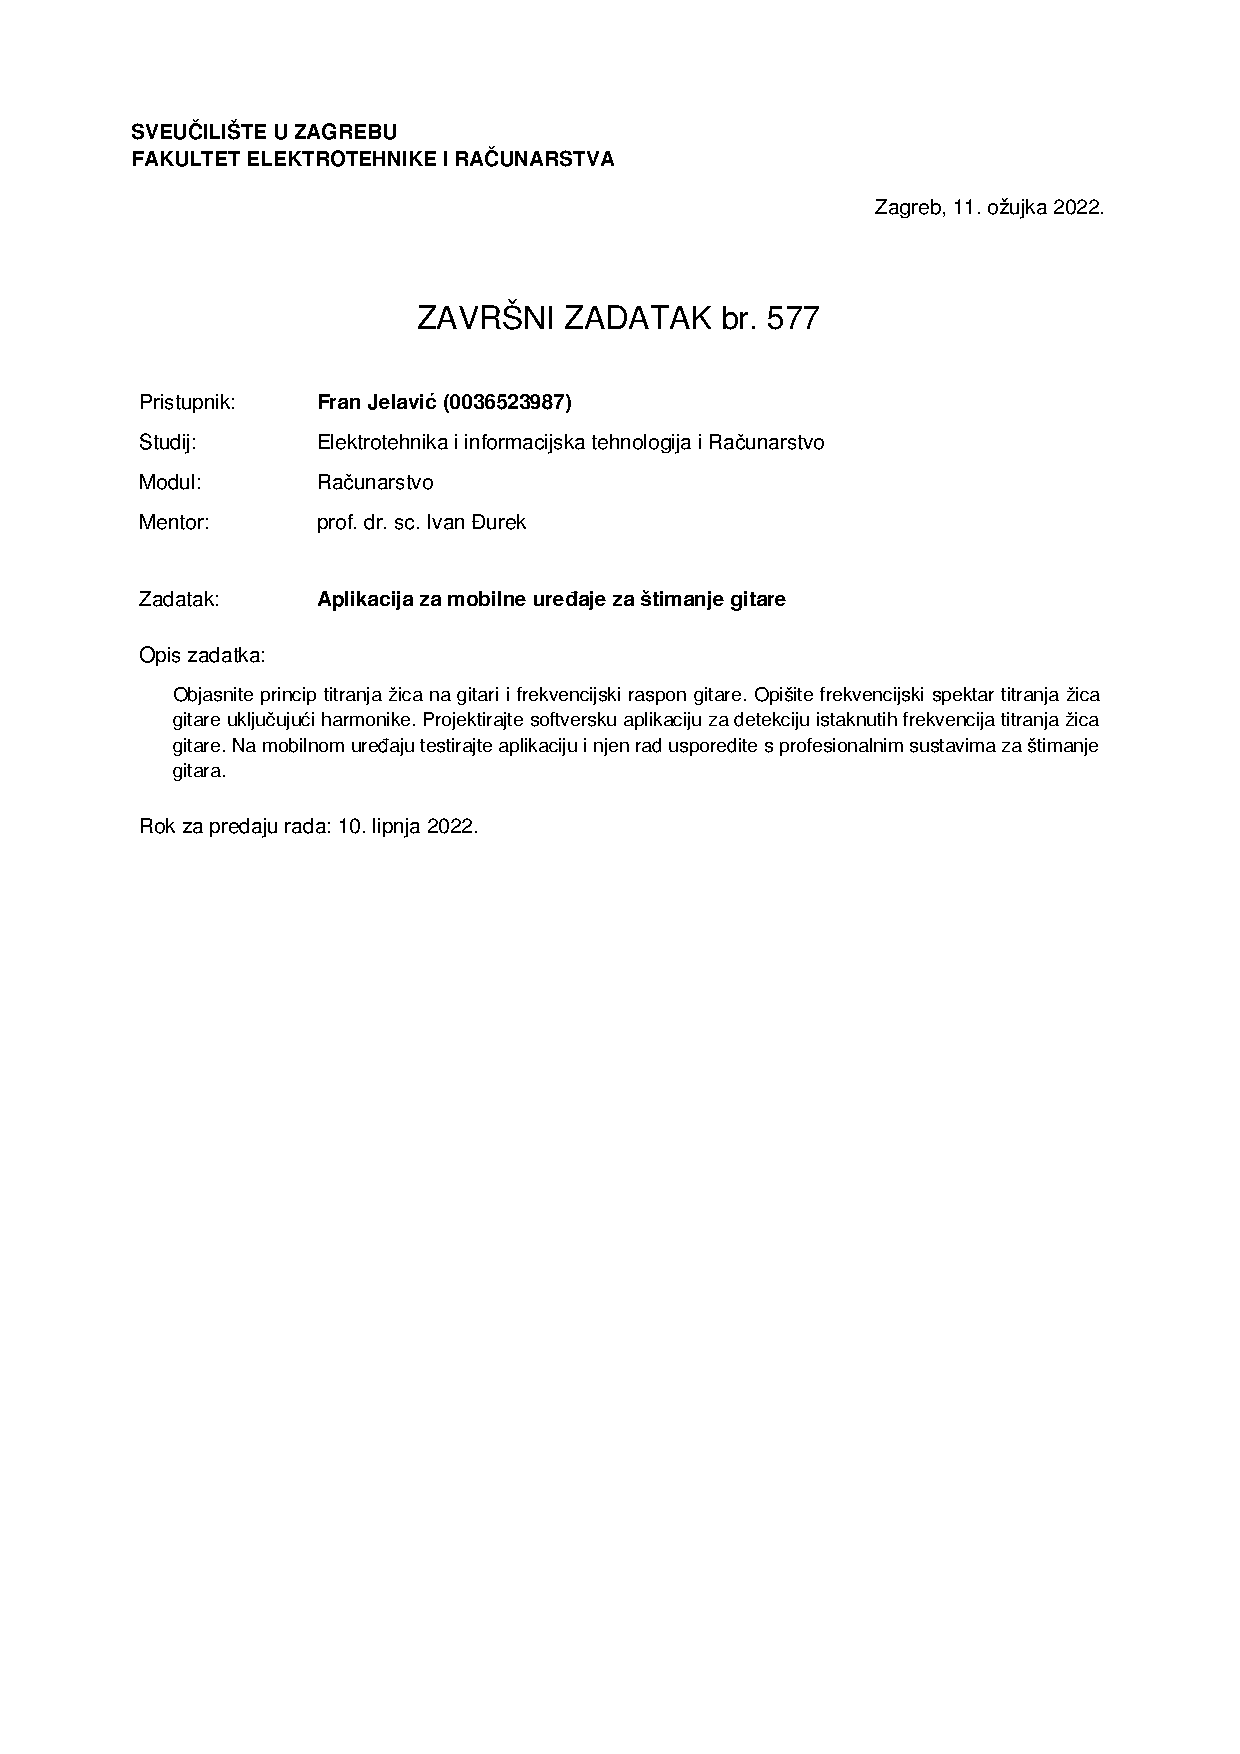
\includepdf[pages={1}]{izvornik.pdf}

% Dodavanje zahvale ili prazne stranice. Ako ne želite dodati zahvalu, naredbu ostavite radi prazne stranice.
\zahvala{Zahvala mentoru prof. dr. sc. Ivanu Đureku što je pružio mogućnost vlastitog izbora teme i dopustio rad vlastitim tempom.}

\tableofcontents

\chapter{Uvod}
%Uvod rada. Nakon uvoda dolaze poglavlja u kojima se obrađuje tema. 1 do 2 strane
Digitalna obrada signala često se koristi za obradu zvuka u glazbenoj umjetnosti. Svaki glazbeni instrument na drugačiji način proizvodi zvuk, ali svaki glazbeni instrument funkcionira po istim principima titranja.
Njihova konzistentnost u proizvodnji frekvencija titranja omogućava jednostavniju obradu zvučnog signala iz zvučnih snimki instrumenata. 

Ovaj rad temelji se na detekciji frekvencija titranja u stvarnome vremenu uz primjer gitare. Jedan od mogućih načina implementacija detekcije frekvencija i obrade zvučnog signala bit će prikazana pomoću aplikacije za štimanje gitare na mobilnim uređajima.

%

\chapter{Frekvencija i visina tona}
%Frekvencija, zvučni valovi, visina tona...
Zvučni val, kao svaki longitudinalni val, unosi se u medij titranjem objekta. Izvor vala je objekt koji titra, a medij je okruženje kojim val prolazi. Titrajući objekt u kontekstu zvučnih valova mogu biti glasnice čovjeka, žica koja titra, zvučnik itd. Medij u ovom kontekstu je zrak, ljudsko uho, i slično. Bez obzira koji objekt stvara zvučni val, čestice medija kroz koji val prolazi gibaju se naprijed-nazad (sabijaju i razrjeđuju) pri određenoj frekvenciji.

Frekvencija vala odnosi se na to koliko često čestice medija vibriraju kada val prođe kroz medij. Mjeri se kao broj potpunih titraja (kompresija) čestice medija u jedinici vremena. Drugim riječima, mjeri se u titrajima po sekundi, tj. hercima (Hz).

Kako se zvučni val kreće kroz medij, svaka čestica medija titra pri istoj frekvenciji, budući da svaka čestica titra radi gibanja svog najbližeg susjeda. Isto tako, frekvencija na kojoj vibrira svaka čestica vala jednaka je frekvenciji izvora zvučnog vala. Primjerice, žica gitare koja titra pri frekvenciji od 500 Hz će uzrokovati da čestice u okruženju titraju pri istoj frekvenciji od 500 Hz, što će rezultirati prenošenjem zvučnog vala frekvencije od 500 Hz do uha slušatelja.

Poznato je da se raspon frekvencija koju mogu raspoznati ljudi proteže između 20 Hz do 20 kHz.

\section{Visina tona}
Visina tona (eng. \textit{pitch}) je termin koji se često koristi kao sinonim za frekvenciju. Iako su vrijednosti izravno povezane i proporcionalne, frekvencija mjeri titraj fizičkog vala u jedinici vremena, dok se visina tona koristi za ljudsku percepciju zvuka (najčešće u glazbi).\cite{stevens1940relation}

Viša frekvencija odgovara višoj visini tona, kao što i niža frekvencija odgovara nižoj visini tona. Većina ljudi može raspoznati dva istovremena zvuka s razlikom frekvencija od 7 Hz, dok neki i do 2 Hz.

%

\chapter{Frekvencija u glazbi}
%Frekvencija u glazbi, kromatska ljestvica, note...
Ljestvica u zapadnjačkoj koncertnoj glazbi temelji se na oktavi, što je razlika između dva zvuka čije su frekvencije u omjeru 2:1. Dva tona odsvirana istovremeno s razlikom u oktavi zvuče ugodno, stoga oktava ima široku primjenu u glazbi. 

Kromatska ljestvica (eng. chromatic scale ili twelve-tone scale) sačinjena je od jedne oktave podijeljene na 12 jednakih intervala, pri čemu svi intervali imaju jednaki omjer frekvencija od $\sqrt[12]{2}$, odnosno svaki interval je udaljen za jedan poluton (eng. \textit{semitone}).\cite{sundberg1982tune}

\section{Glazbene note}
U glazbi se termin nota koristi za reprezentaciju određene visine (i duljine u zapisu) tona. Nota se ujedno koristi i za skupinu visine tona koje spadaju u isti razred (eng. \textit{pitch class}), tj. visine tonova koje su odvojene oktavom. U regijama u kojima se govori engleski uglavnom se koristi zapis nota kojim su note predstavljene pomoću prvih sedam slova latinske abecede (A, B, C, D, E, F i G). Osma nota, nazvana oktavom, zapisuje se istim nazivom (slovom) kao prva, ali ima dvostruko višu frekvenciju. 

Kako bi se razlikovale dvije note istog razreda, ali različitih oktava, sustav znanstvenog zapisa visine tona (eng. \textit{scientific pitch notation}) kombinira naziv note s brojem koji označava određenu oktavu. 
Primjerice, $E_2$ s frekvencijom od 82,41 Hz je za jednu oktavu viša od $E_1$ s frekvencijom od 41,20 Hz, a za dvije oktave viša od $E_0$ s frekvencijom od 20,60 Hz.

Uz broj, nazivu note može se pripisati predznak akcidental (eng. \textit{accidental}).\cite{pericic2008visejezicni} Pod akcidentale spada znak povisilice (eng. \textit{sharp} - $\sharp$) koji podiže notu na frekvenciju koja je $\sqrt[12]{2}$ puta veća od trenutne te znak snizilice (eng. \textit{flat} - $\flat$) koji spušta notu na frekvenciju $\sqrt[12]{2}$ puta manju od trenutne. Drugim riječima, povisilica ($\sharp$) podiže notu za jedan poluton, dok snizilica ($\flat$) spušta notu za jedan poluton.\cite{hemu_2020}
Primjerice, $F_4^\sharp$ s frekvencijom od 369,99 Hz je za jedan poluton viši od $F_4$ s frekvencijom od 349,23 Hz, ali isto tako za jedan poluton niži od $G_4$ s frekvencijom od 392 Hz. Stoga se nota $F_4^\sharp$ da zapisati i kao $G_4^\flat$.

Osim povisilice ($\sharp$) i snizilice ($\flat$), pod akcidentale se ubraja i razrešnica (eng. \textit{natural} - $\natural$), koji se pridodaje tzv. prirodnoj noti čija visina tona ostaje nepromijenjena, odnosno nije ni povišena ni snižena za poluton.\cite{benward2003introduction} Ovaj akcidental se uglavnom ne koristi jer se bez njegovog dodatka nazivu note sporazumijeva da je nota prirodna.

\section{Kromatska ljestvica}
Konačno, uz navedene informacije može se prikazati kromatska ljestvica, konstruirana po noti C.

%C & C$\sharp$ ili D$\flat$ & D & D$\sharp$ ili E$\flat$ & E & F & F$\sharp$ ili G$\flat$ & G & G$\sharp$ ili A$\flat$ & A & A$\sharp$ ili B$\flat$ & B\\
\begin{center}
	\begin{tabular}{c c c c c c c c c c c c}
		$C$ & $C^\sharp$ ili $D^\flat$ & $D$ & $D^\sharp$ ili $E^\flat$ & $E$ & $F$ & $F^\sharp$ ili $G^\flat$ & $G$ & $G^\sharp$ ili $A^\flat$ & $A$ & $A^\sharp$ ili $B^\flat$ & $B$\\
	\end{tabular}
\end{center}

\section{Koncertna visina tona}
Koncertna visina tona (eng. \textit{concert pitch}) je referenca prema kojoj se skupina glazbenih instrumenata štima za nastup. Koncertna visina tona može varirati od ansambla do ansambla, a često se mijenjala kroz povijest. Najčešći moderni standard za štimanje koristi 440 Hz za notu $A_4$, prema kojoj se u odnosu na nju ostale note postavljaju.

\section{Intervali u glazbi}
U glazbi se termin intervala koristi za razliku u visini tona između dva zvuka.\cite{prout2011harmony} Najmanji interval kromatske ljestvice je poluton. Pri početku poglavlja spomenuto je da su frekvencije dviju nota s razlikom u oktavi u omjeru 2:1. To znači da se uzastopnim povećanjem visine tona za isti interval ujedno eksponencijalno povećava frekvencija, iako ljudsko uho to percipira kao linearno povećanje visine tona. Iz tog razloga, intervali se često mjere u centima (eng. \textit{cent}).\cite{benson2006music} Cent je jedinica dobivena dijeljenjem polutona na 100 jednakih dijelova, odnosno dijeljenjem oktave na 1200 jednakih dijelova.  Formulu za cent moguće je izraziti logaritmom omjera frekvencija:

\begin{equation}
	n = 1200 * \log_2(\dfrac{f_1}{f_2}) \\ 
\end{equation}

pri čemu je $n$ broj izražen u centima (cent), a $f_1$ i $f_2$ frekvencije izražene u hercima (Hz).

\section{Harmonici}
Većina zvukova mješavina je različitih frekvencija. Pregibi ili harmonici (eng. \textit{harmonics}) nastaju pri zvukovima s jednom dominantnom, odnosno temeljnom frekvencijom (eng. \textit{fundemental frequency}), kao frekvencije višekratnika temeljne frekvencije.\cite{sethares2005tuning} Temeljna frekvencija je najniža frekvencija kojom objekt titra i uglavnom je najvećeg intenziteta.\cite{teachmeaudio2020} Primjerice, ako je $F$ temeljna frekvencija, harmonike zvuka bi se moglo prikazati na ovaj način:

\begin{equation}
	a*F + b*2F + c*3F + ...\\
\end{equation}

pri čemu su $a$, $b$, $c$ koeficijenti intenziteta. Koeficijent $a$ je uglavnom najveći, budući da je $F$ temeljna frekvencija. Razliku u koeficijentima čine različiti izvori zvuka. Osim intenziteta harmonika, razliku u zvuku između dvaju različita izvora čine i slabije popratne frekvencije, tzv. alikvotne tonove (eng. \textit{overtones}) koji tonu daju dodatnu boju.\cite{christensen1987science} Iz tih razloga će nota odsvirana na dva različita instrumenta zvučati drugačije, ali jednake visine tona.

Više o harmonicima objašnjeno je u sljedećem poglavlju, na primjeru titranja žica gitare.

%

\chapter{Frekvencije na primjeru gitare}
%gitara
Ovaj rad služi se isključivo primjerom standardno naštimane (eng. \textit{standard tuning}) akustične gitare, prema standardnoj koncertnoj visini tona (440 Hz). \textit{Standard tuning} podrazumijeva da su žice, od gornje prema donjoj, redom naštimane prema notama $E_2$, $A_2$, $D_3$, $G_3$, $B_3$ i $E_4$.

\section{Frekvencijski raspon}
Frekvencijski raspon gitare ovisi o tome kako je gitara štimana i o samom tipu gitare (klasična, akustična, električna) budući da različiti tipovi gitare imaju različitu građu (posebice duljinu vrata).

Frekvencijski raspon akustične gitare proteže se od note $E_2$ s frekvencijom od 82,41 Hz do note $C_6^\sharp$ s frekvencijom od 1108,73 Hz. Valja napomenuti da je najniža frekvencija postignuta sviranjem "otvorene" (nepritisnute) gornje $E_2$ žice, a najviša frekvencija postignuta sviranjem donje $E_4$ žice, pritisnute na 21. polju (eng. \textit{fret}) vrata gitare.

\clearpage

\begin{table}
	\begin{center}
		\begin{tabular}{c|c c c c c}
			Nota/oktava  & 2 & 3 & 4 & 5 & 6\\
			\hline
			$C$ & & 130,8 & 261,6 & 523,3 & 1047\\
			\hline
			$C^\sharp$ &  & 138,6 & 277,2 & 554,4 & 1109\\
			\hline
			$D$ & & 146,8 & 293,7 & 587,3 & \\
			\hline
			$D^\sharp$ & & 155,6 & 311,1 & 622,3 & \\
			\hline
			$E$ & 82,41 & 164,8 & 329,6 & 659,3 & \\
			\hline
			$F$ & 87,31 &174,6 & 349,2 & 698,5 & \\
			\hline
			$F^\sharp$ & 92,50 & 185,0 & 370,0 & 740,0 & \\
			\hline
			$G$ & 98,00 & 196,0 & 392,0 & 784,0 & \\
			\hline
			$G^\sharp$ & 103,8 & 207,7 & 415,3 & 830,6 & \\
			\hline
			$A$ & 110,0 & 220,0 & 440,0 & 880,0 & \\
			\hline
			$A^\sharp$ & 116,5 & 233,1 & 466,2 & 932,3 & \\
			\hline
			$B$ & 123,5 & 246,9 & 493,9 & 987,8 & \\
		\end{tabular}
		\caption{Frekvencijski raspon akustične gitare u Hz.}
	\end{center}
\end{table}

\section{Frekvencijski spektri}
Harmonici se lako mogu istaknuti prikazima frekvencijskih spektara snimljenih zvukova. Slike 4.1 do 4.6 predstavljaju spektrograme frekvencija žica gitare, snimljene pomoću aplikacije \textit{Spectroid}. Lako je uočiti kako se među frekvencijama ističe temeljna frekvencija i njezini harmonici.

Primjerice, slika 4.5 vrlo jasno prikazuje ovaj fenomen, s istaknutom dominantnom frekvencijom od 247 Hz, što je upravo temeljna frekvencija note $B_3$. Temeljnu frekvenciju redom slijede istaknute frekvencije od 494 Hz, 739 Hz, 985 Hz te 1478 Hz, kao (približni) višekratnici temeljne frekvencije. Valja napomenuti da intenzitet harmonika nije uvijek silazan, što se vidi s harmonikom od 1478 Hz koji je jačeg intenziteta od prethodnih dva harmonika.

Drugačiji primjer pokazuje slika 4.1. Frekvencija od 83 Hz note $E_2$ je istaknuta, ali nije najistaknutija frekvencija. To je česti problem pri detekciji frekvencija iz zvučnih signala. Ovisno o podatcima snimljenog signala, temeljna frekvencija može, ali ne mora biti najistaknutija.\cite{gustine_2021} Više o ovom problemu nastavlja se u poglavlju 6.2.

Zbog neidealnih uvjeta pri mjerenju u sklopu ovoga rada dolazi do slabe devijacije u vrijednostima višekratnika, ali je pojava harmonika svejedno jasno vidljiva.

\clearpage

\begin{figure}
	\centerline{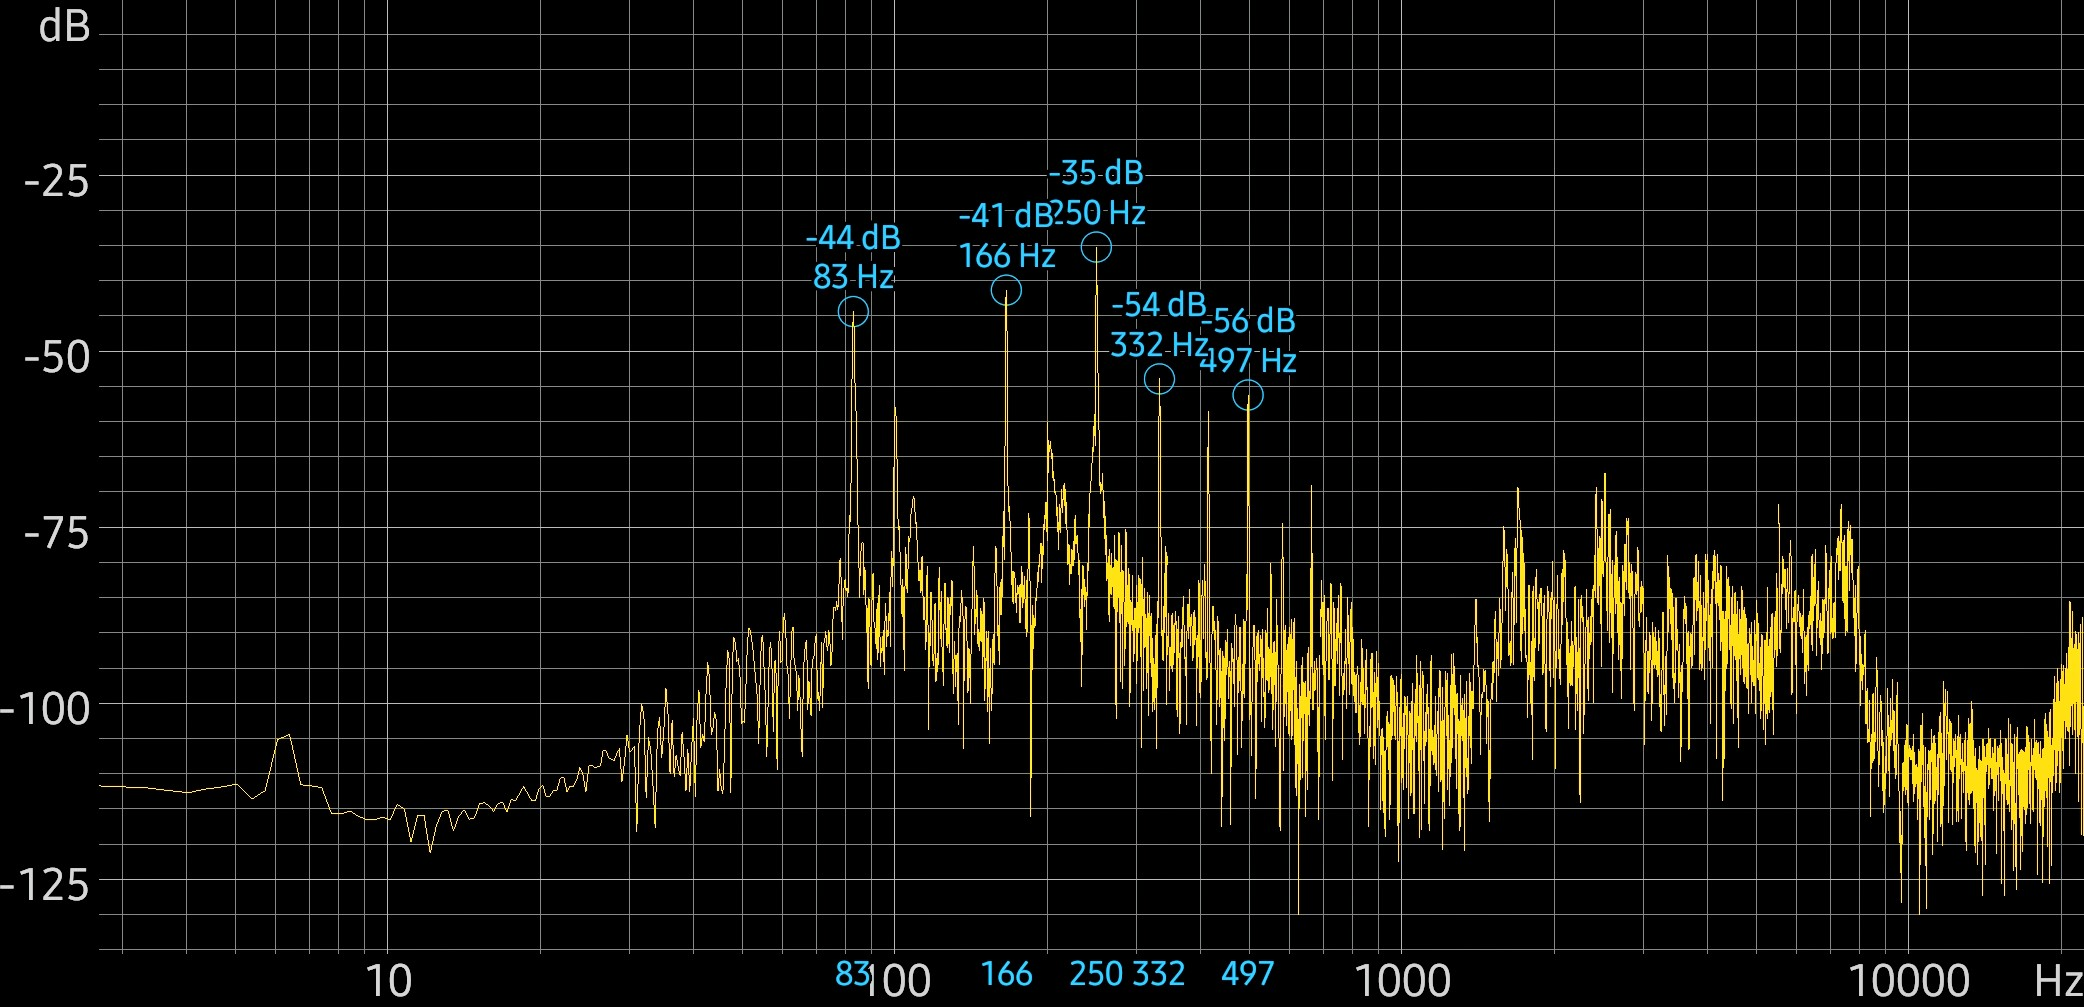
\includegraphics[width=1\textwidth]{spektrogram_e2.jpg}}
	\caption{Frekvencijski spektar žice $E_2$}
	\label{fig}
\end{figure}
\begin{figure}
	\centerline{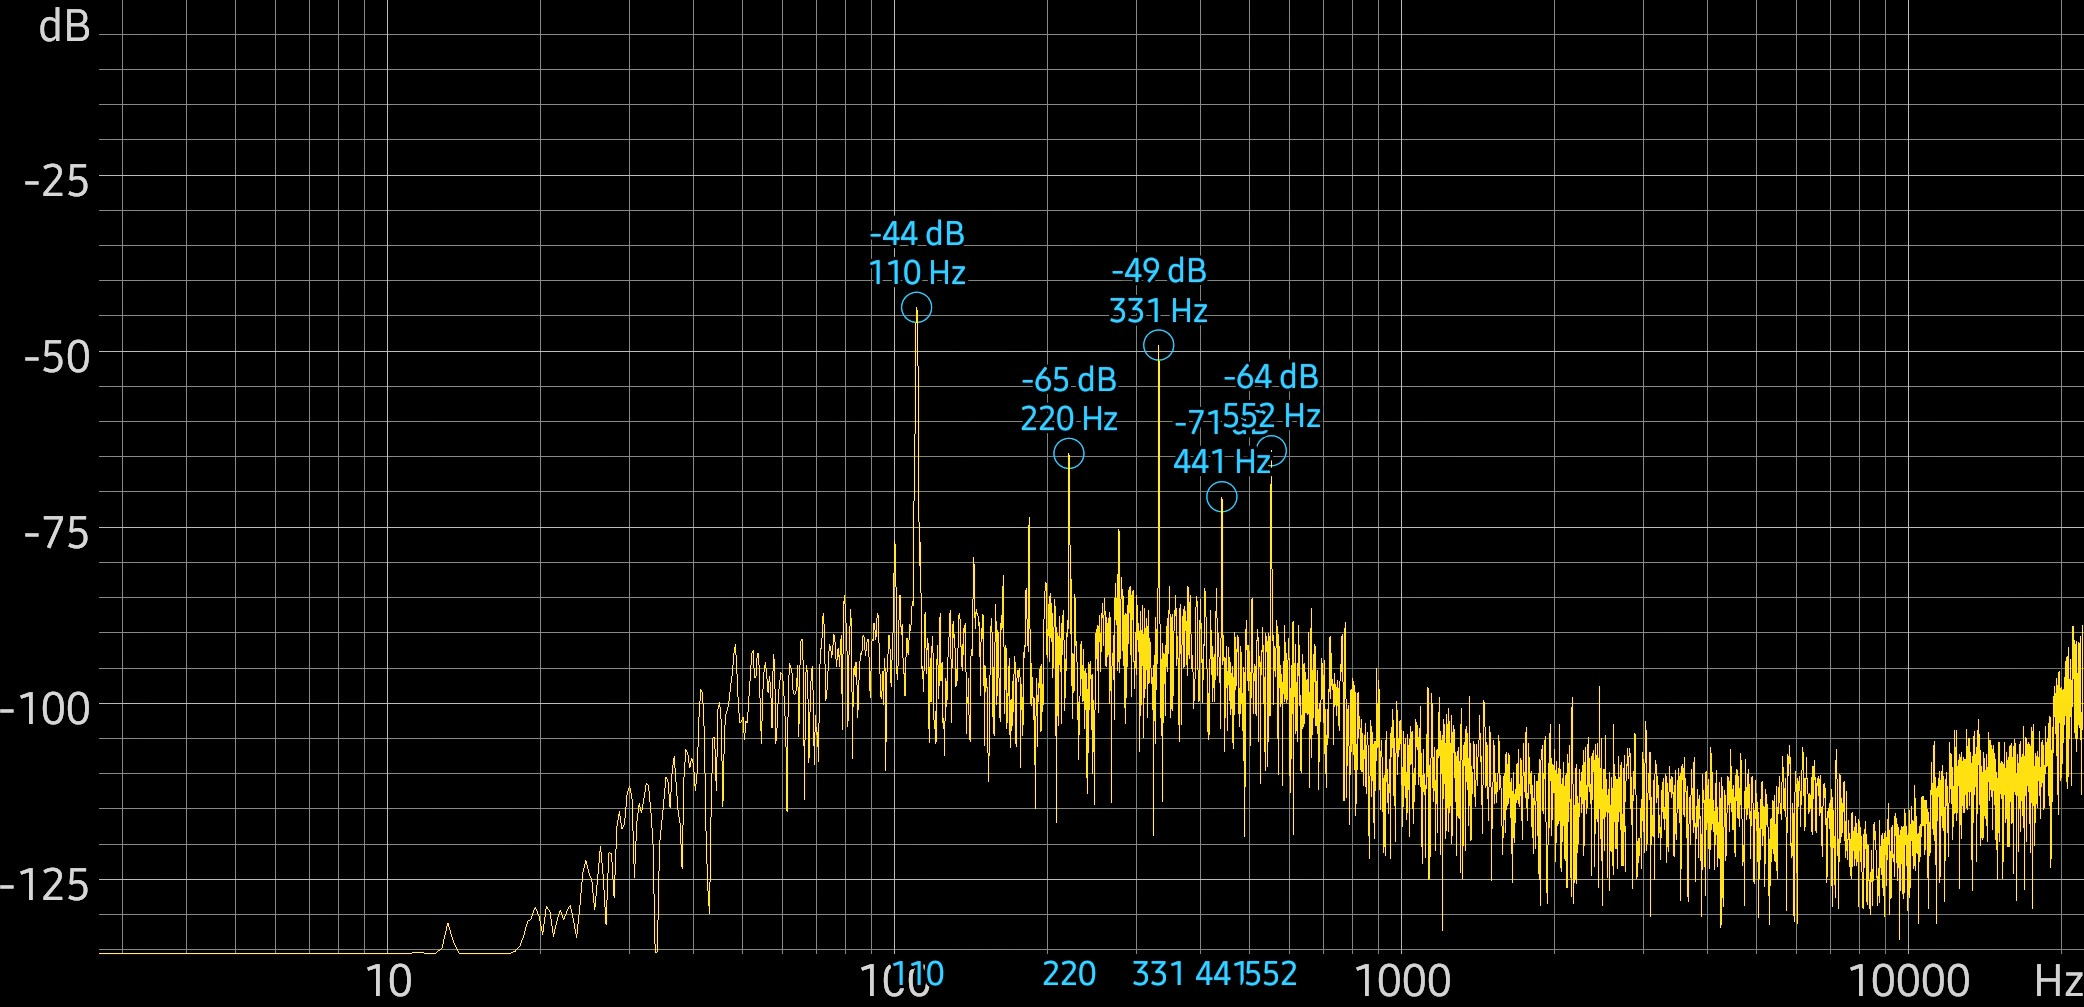
\includegraphics[width=1\textwidth]{spektrogram_a2.jpg}}
	\caption{Frekvencijski spektar žice $A_2$}
	\label{fig}
\end{figure}
\begin{figure}
	\centerline{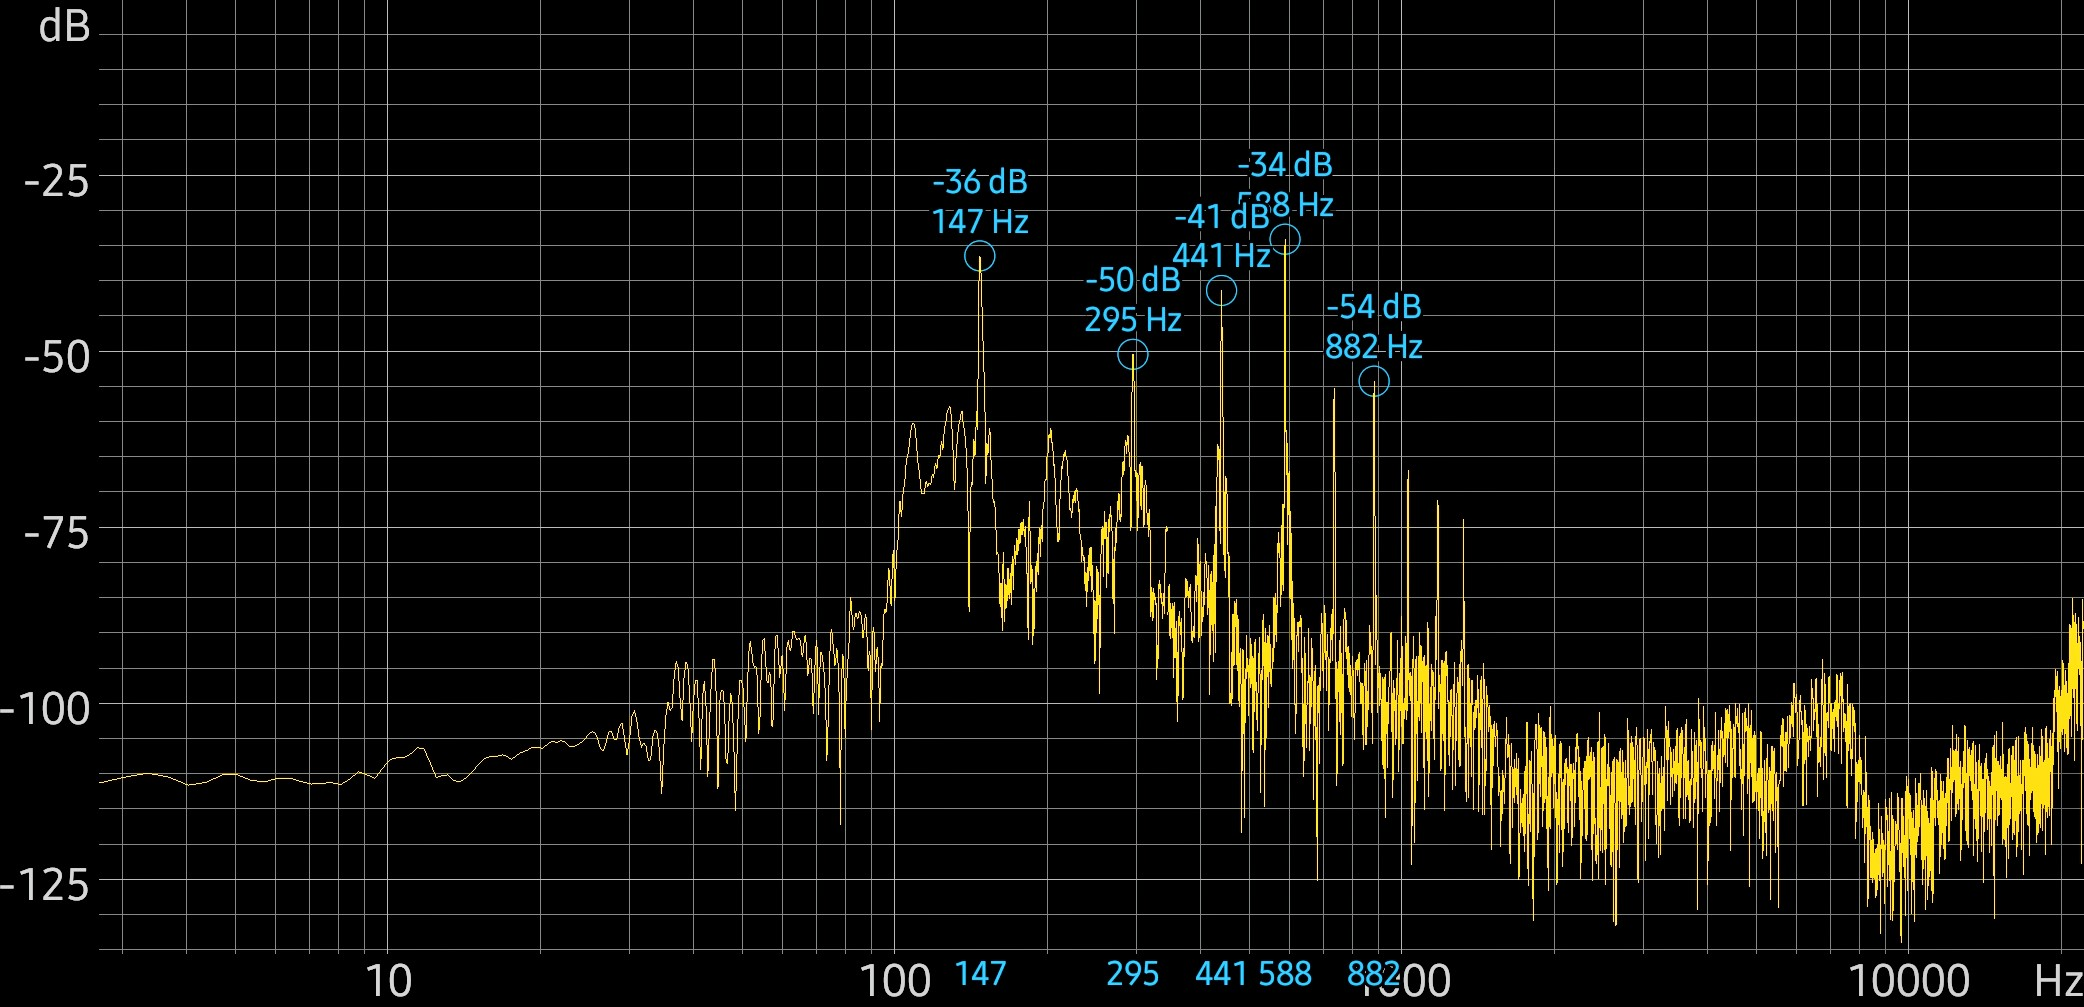
\includegraphics[width=1\textwidth]{spektrogram_d3.jpg}}
	\caption{Frekvencijski spektar žice $D_3$}
	\label{fig}
\end{figure}
\begin{figure}
	\centerline{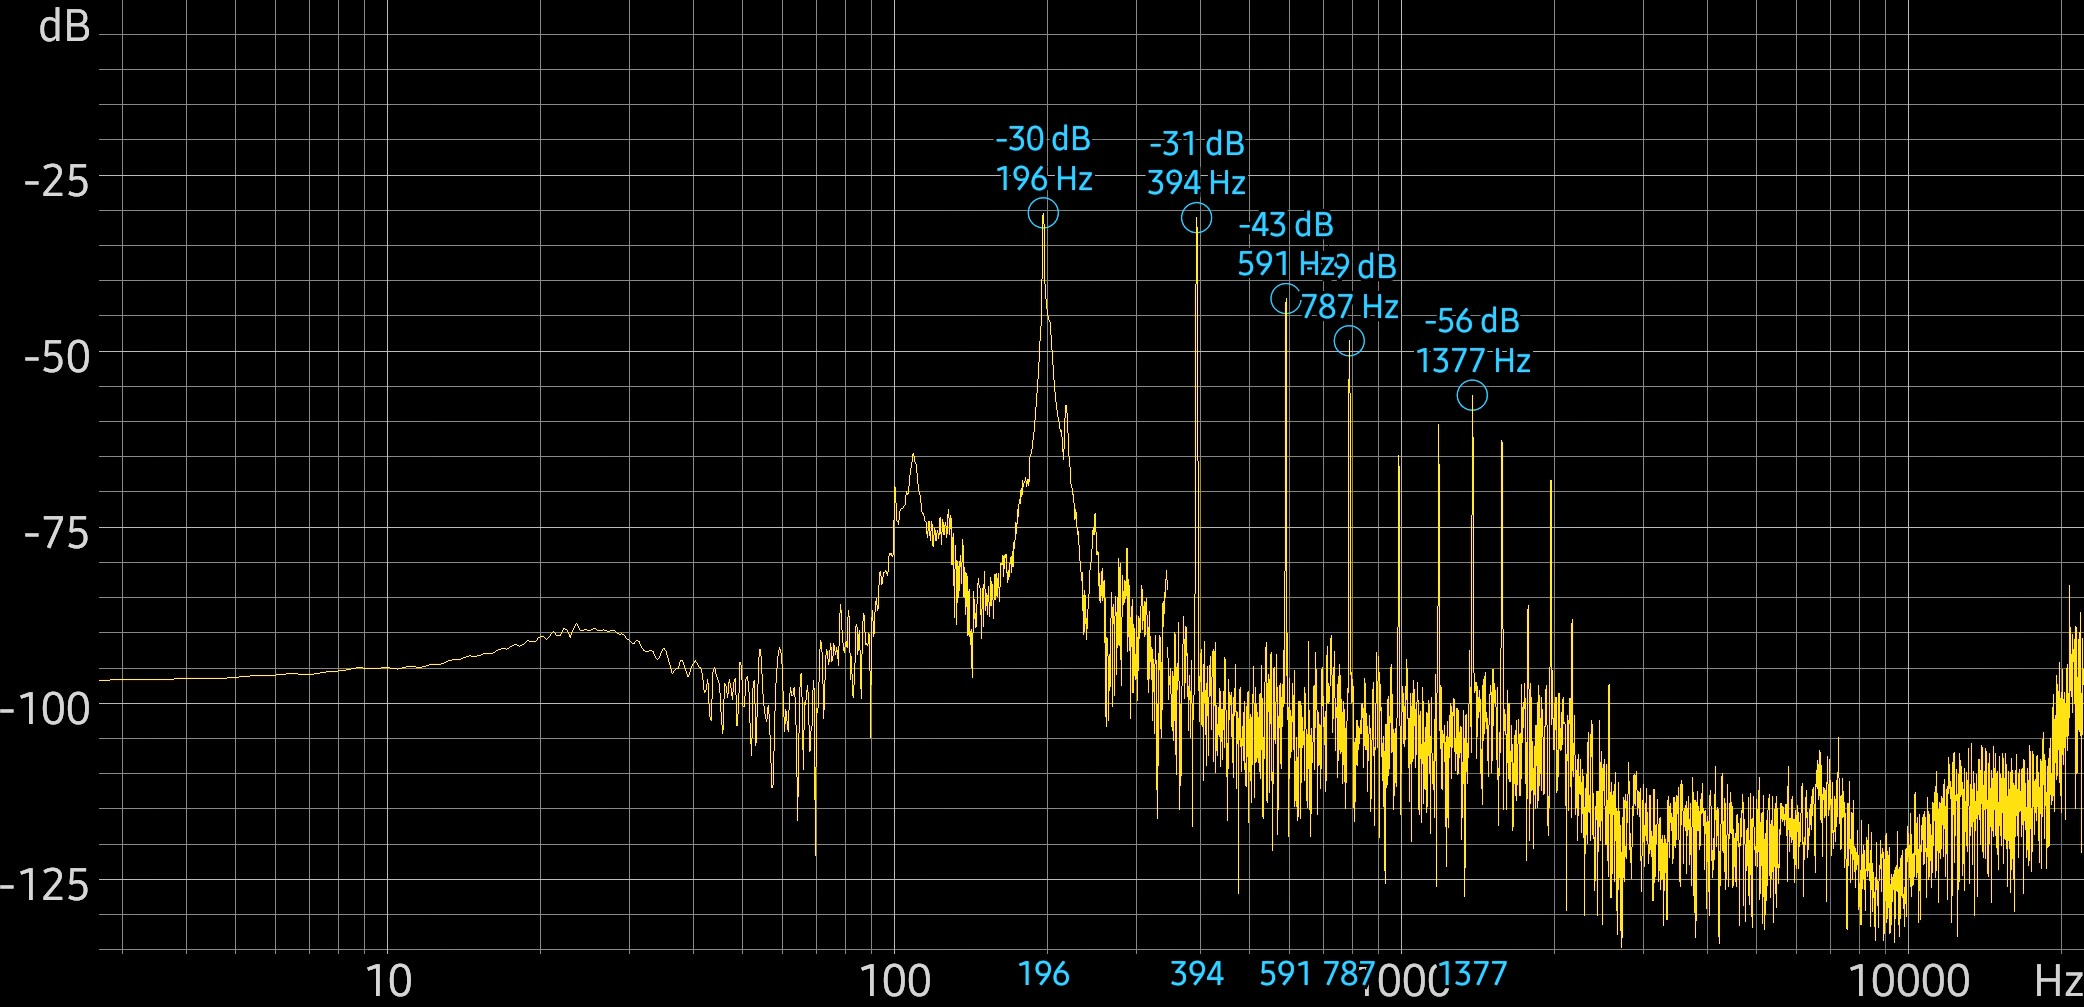
\includegraphics[width=1\textwidth]{spektrogram_g3.jpg}}
	\caption{Frekvencijski spektar žice $G_3$}
	\label{fig}
\end{figure}
\begin{figure}
	\centerline{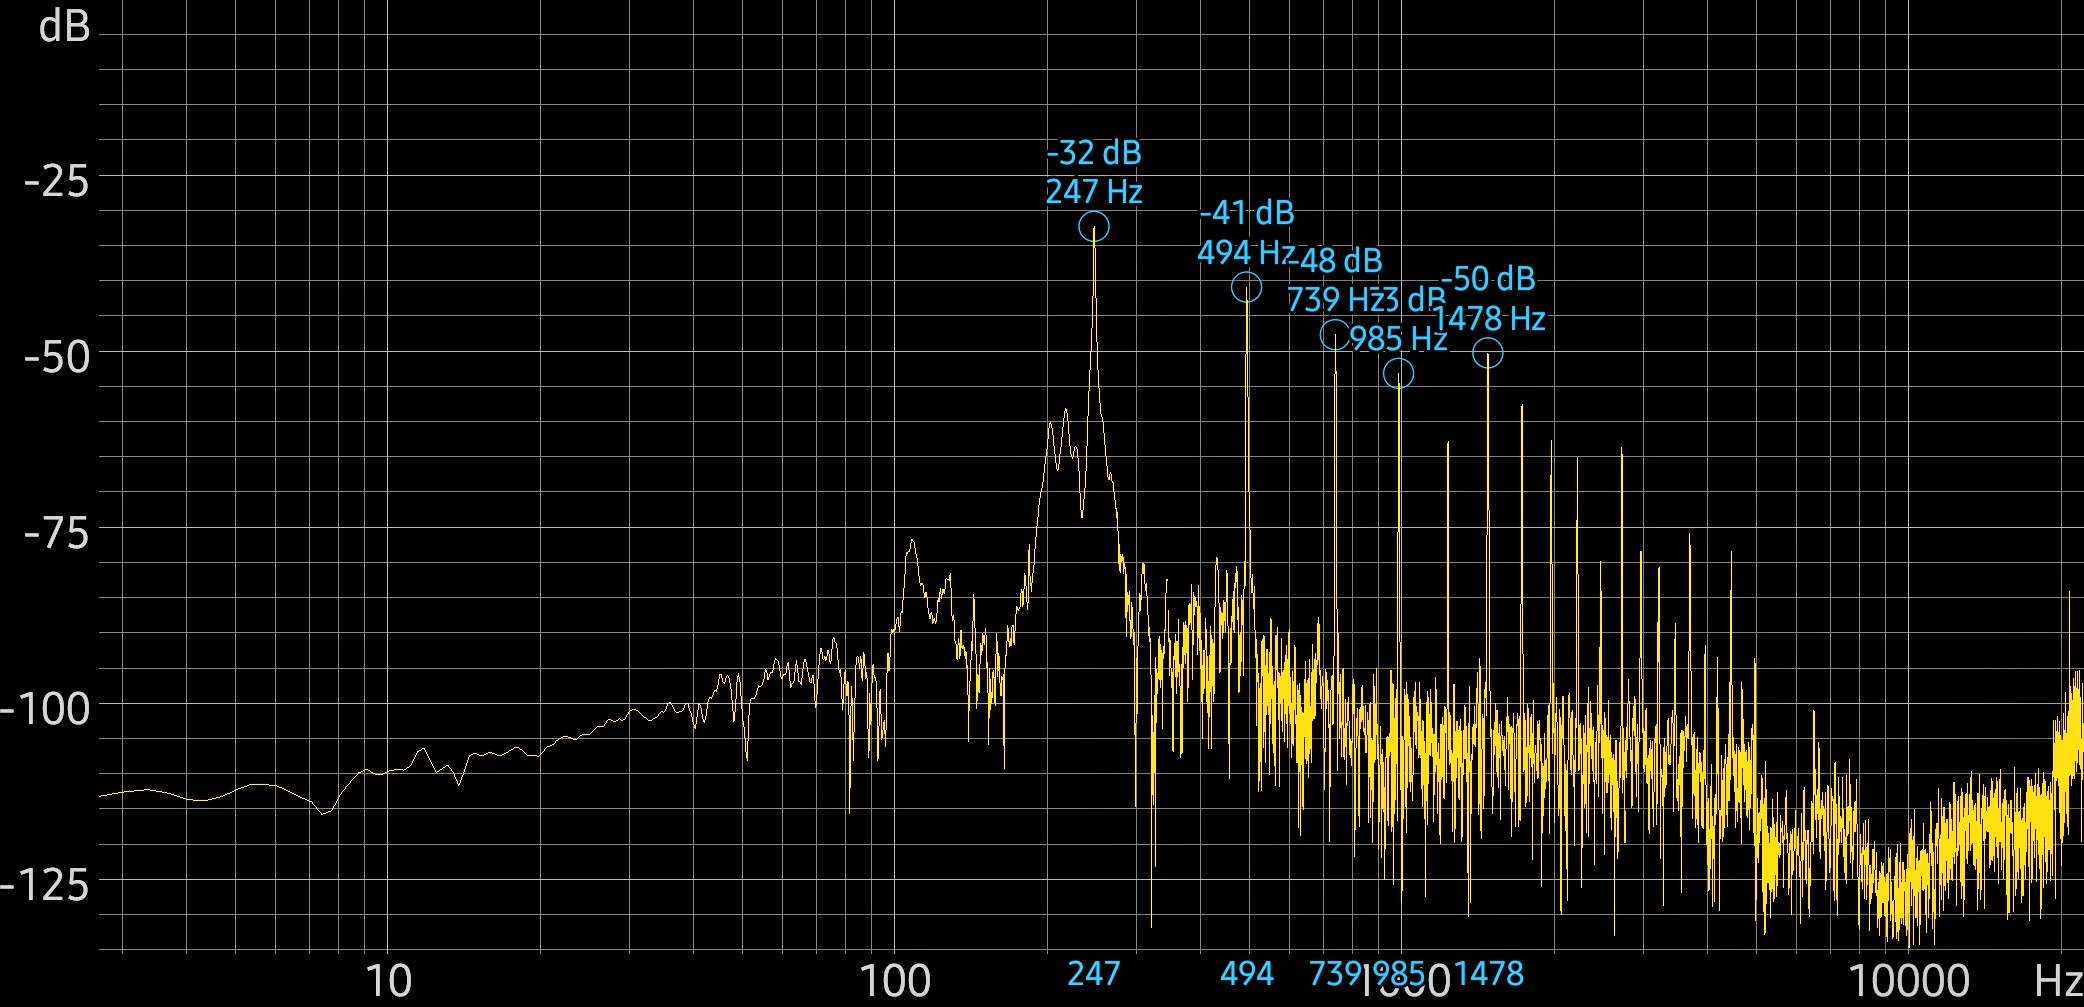
\includegraphics[width=1\textwidth]{spektrogram_b3.jpg}}
	\caption{Frekvencijski spektar žice $B_3$}
	\label{fig}
\end{figure}
\begin{figure}
	\centerline{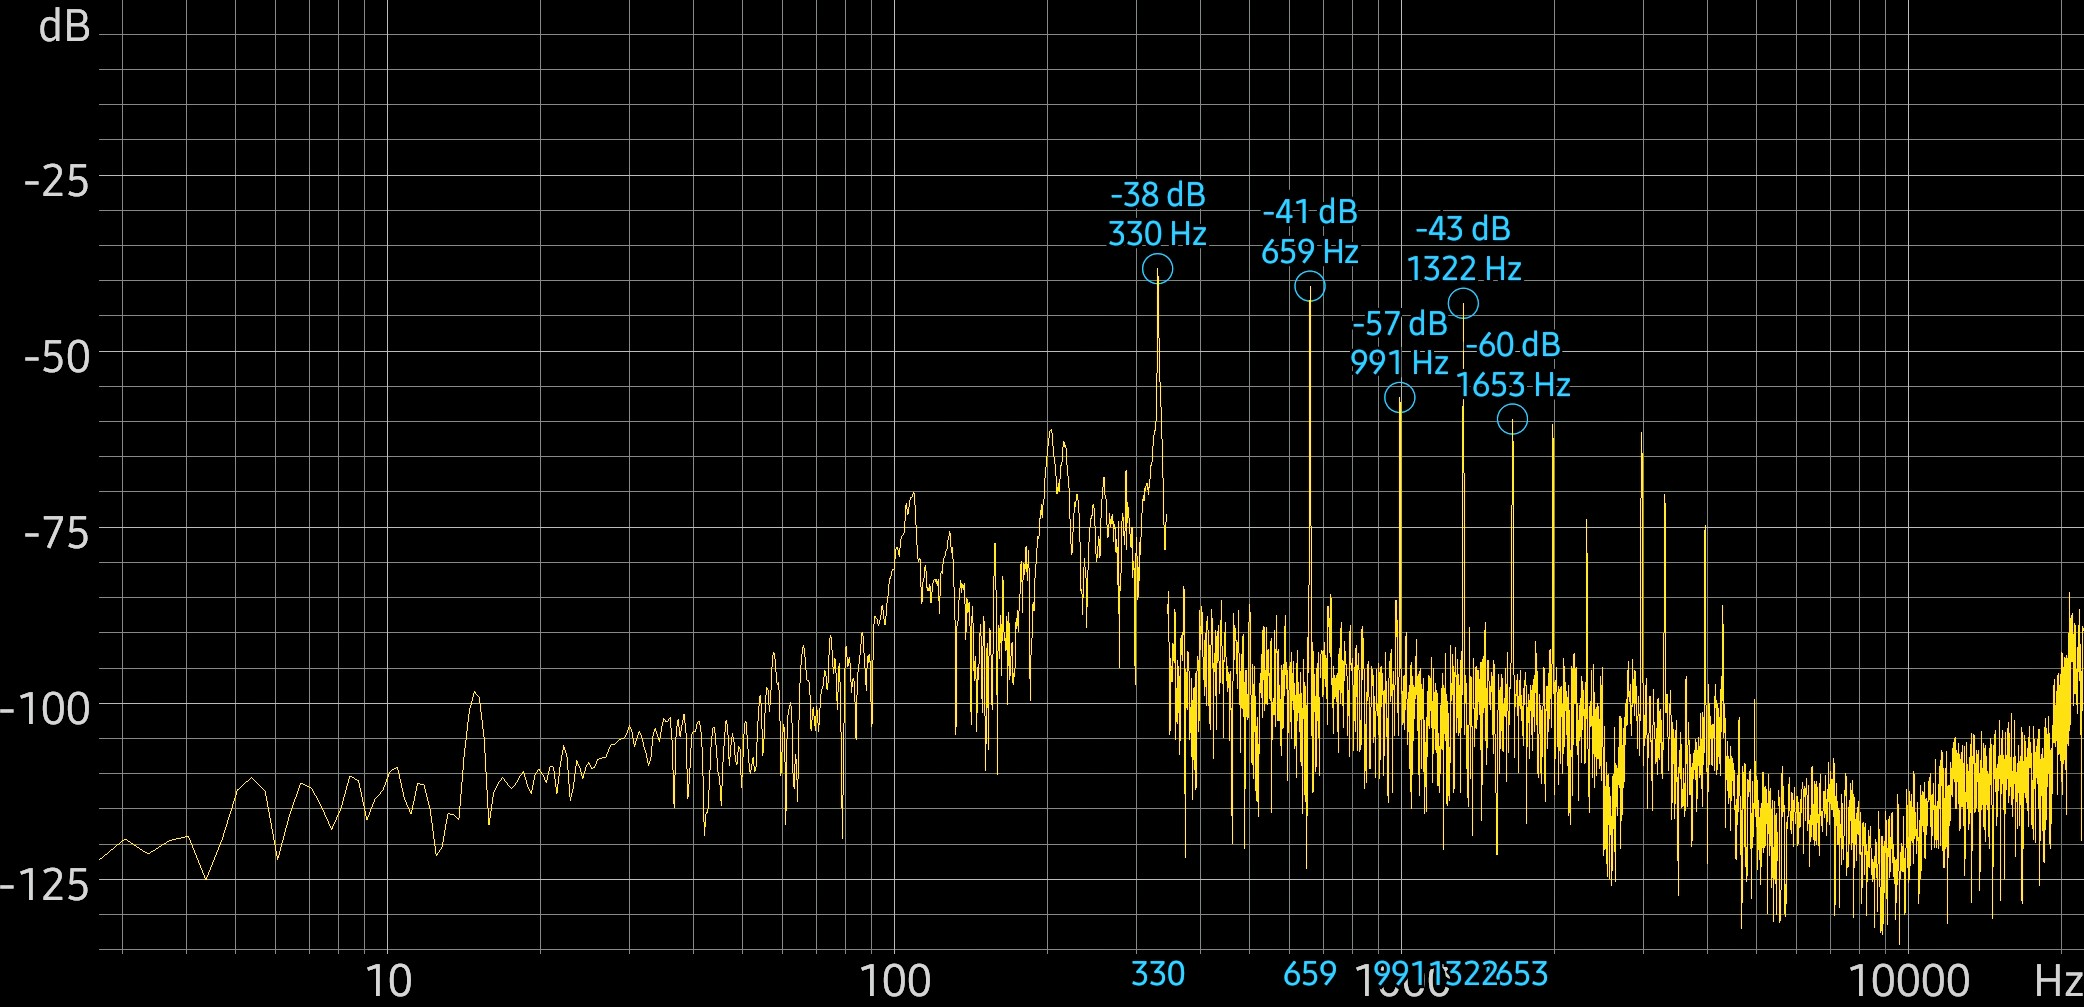
\includegraphics[width=1\textwidth]{spektrogram_e4.jpg}}
	\caption{Frekvencijski spektar žice $E_4$}
	\label{fig}
\end{figure}

%

\chapter{Digitalna obrada signala}
%O samoj digitalnoj obradi signala
Digitalna obrada signala (eng. \textit{Digital Signal Processing} - \textit{DSP}) koristi procesore signala koji preuzimaju snimljene signale iz stvarnog svijeta poput zvuka, govora, video prikaza, temperature, tlaka, radara ili ostalih signala koji su digitalizirani te nad njima izvode matematičke operacije kako bi ih oblikovali.

Signale je potrebno obraditi kako bi se informacija koju sadrže mogla bolje prikazati, analizirati ili pretvoriti u drugu vrstu signala koja bi mogla biti od koristi. Kako bi signal uopće bio digitaliziran, potrebno je pretvoriti snimljeni analogni signal u digitalni binarni zapis, što se postiže analogno-digitalnim pretvaračima (eng. \textit{Analog-to-digital converter} - \textit{ADC}).

Primjena digitalne obrade signala omogućuje mnoge prednosti u odnosu na analognu obradu, kao što je kompresija podataka ili otkrivanje i ispravljanje pogrešaka pri prijenosu podataka.\cite{broesch2008digital}

U ovome radu digitalna obrada signala odnosi se isključivo na obradu snimljenog zvučnog signala.

\section{Uzorkovanje}
%Sampling
U kontekstu obrade zvučnog signala, uzorkovanje (eng. \textit{sampling}) je pretvorba zvučnog vala u slijed "uzoraka". Uzorak (eng. \textit{sample}) je vrijednost signala u točki u vremenu i/ili prostoru. Sklop za uzorkovanje (eng. \textit{Sampler}) je operacija ili sustav koji izvlači uzorke iz "kontinuiranog" signala. Cilj sklopa za uzorkovanje je zabilježiti uzorke ekvivalentne njihovim trenutnim vrijednostima u signalu. 

Frekvencija uzorkovanja (eng. \textit{sample rate} ili \textit{sampling frequency}) je prosječni broj dobavljenih uzoraka u jednoj sekundi te se mjeri u hercima (Hz). Frekvencija uzorkovanja je najčešće iznad 40 kHz radi teorema Nyquista i Shannona, koji tvrdi da je rekonstrukcija signala moguća tek kada je frekvencija uzorkovanja dvostruka veća od frekvencije signala koji se obrađuje.\cite{candes2008introduction} Zvučni signali snimljeni su uglavnom do 20 kHz, budući da je to gornja granica ljudskog sluha.

Najčešće frekvencije uzorkovanja su 44,1 kHz, 48 kHz, 88,2 kHz ili 96 kHz.\cite{self2012audio} Koriste se uglavnom frekvencije uzorkovanja do 50 kHz jer vrijednosti više od toga ne pridonose zvuku za ljudsko uho, a zauzimaju veću širinu pojasa (eng. \textit{bandwidth}).

\chapter{Algoritam brze Fourierove transformacije - FFT}
%FFT
Aplikacija \textit{Spectroid} za detekciju frekvencija koristi algoritam brze Fourierove transformacije (eng. \textit{Fast Fourier Transform} - \textit{FFT}).\cite{reinke_2018} Algoritam FFT pretvara signal u skup brojeva pomoću kojeg se da raspoznati najzastupljenije frekvencije u signalu. Sposobnost FFT-a da podijeli zvučni signal u frekvencije od kojih se sastoji ga čini jako korisnom metodom koja se često koristi u praksi obrade zvučnih signala.\cite{gustine_2021}

\section{Način rada FFT-a}
%nacin rada fft
Obradom signala pomoću FFT-a, na izlazu se dobiva slijed brojeva u nizu koji predstavlja domenu frekvencija obrađenog signala, npr.:
\begin{verbatim}
	fft_output_array = [23, 43, 65, 443, 321, 54, 56 ...]
\end{verbatim}
Svaki indeks ovog niza naziva se \textit{bin} te predstavlja određen raspon frekvencija. Broj na svakom indeksu je intenzitet frekvencija u rasponu koji predstavlja. Što je broj veći, to je veća zastupljenost frekvencija unutar svoga raspona. Raspon frekvencija u pri svakom indeksu ovisi o rezoluciji (eng. \textit{resolution}) koja se može izraziti na sljedeći način:
\begin{verbatim}
	resolution = sampling_rate / fft_size
\end{verbatim}
pri čemu je \verb|fft_size| veličina spremnika za uzorke (eng. \textit{buffer size}).\cite{lourde2009digital} Veličina \textit{buffer}-a povezana je s vremenom koje je potrebno za obradu signala, pri čemu manje veličine stvaraju manje kašnjenje, ali predstavljaju veći teret pri procesiranju i veću mogućnost grešaka.\cite{focusrite_2022}

Kako bi se raspoznale frekvencije po \textit{bin}-ovima, može se koristiti sljedeća formula:
\begin{verbatim}
	start_frequency = bin_number * resolution
\end{verbatim}
pri čemu je \verb|start_frequency| početna frekvencija raspona.\cite{gustine_2021} Raspon frekvencija bi time bio od \verb|start_frequency| do \verb|start_frequency + resolution|.

Primjerice, s frekvencijom uzorkovanja od 48 kHz i veličinom \textit{buffer}-a od 1024 uzoraka dobiva se rezolucija od 46,875 Hz po uzorku; što znači da svaki \textit{bin} predstavlja raspon frekvencija dugačak 46,875 Hz. Prošlom formulom moguće je izračunati početnu frekvenciju raspona 12. \textit{bin}-a, a ta frekvencija je 562,5 Hz. Time se može zaključiti da se raspon 12. \textit{bin}-a proteže od 562,5 Hz do 609,375 Hz.

Kako bi algoritam mogao raspoznati dvije različite note, rezolucija mora biti manja ili jednaka razlici njihovih frekvencija.
U navedenome primjeru izračunata je rezolucija od 46,875 Hz po uzorku. Ako se uspoređuju note najnižih frekvencija akustične gitare ($E_2$ od 82,41 Hz i $F_2$ od 87,31 Hz) gdje je razlika u frekvencijama najniža (4,9 Hz), rezolucija neće biti dovoljno niska da se note mogu raspoznati. Stoga je potrebno sniziti rezoluciju na vrijednost od 4,9 Hz po uzorku ili niže. To je moguće postići snižavanjem vrijednosti frekvencije uzorkovanja ili povećanjem \textit{buffer}-a, po cijeni dodatnog opterećenja procesora i vremena za punjenje \textit{buffer}-a, što u krajnju ruku smanjuje koliko su rezultati u stvarnom vremenu.

\section{Problemi FFT-a}
%problem ffta naveden u 4.2
U poglavlju 4.2 spomenut je problem pri detekciji temeljne frekvencije signala. Na slici 4.1 temeljna frekvencija note $E_2$ je 82,41 Hz, ali nije najvećeg intenziteta. Stoga se ne može pouzdati na prepoznavanje temeljne frekvencije preko one s najvećim intenzitetom. Ova pojava može izazvati veliki problem u sustavu koji bi trebao prepoznati visinu tona odsvirane note.

Budući da algoritam FFT sam po sebi nije dovoljno dobar alat za cilj koji ovaj rad nastoji ostvariti, mora se koristiti kompleksniji algoritam. U primjeru ovog rada, koristit će se algoritam YIN.

\chapter{Algoritam YIN}
YIN (nadahnuto filozofijom \textit{yin} i \textit{yang}) algoritam temelji se na metodi autokorelacije (eng. \textit{autocorrelation function} - \textit{ACF}) s brojnim izmjenama koje se kombiniraju kako bi se spriječila pojava grešaka. Algoritam ima nekoliko poželjnih značajki. Učestalost grešaka je oko tri puta manja od najboljih konkurentskih metoda; algoritam je prikladan za glazbu i visoke tonove te je jednostavan za implementaciju, s niskim kašnjenjem (eng. \textit{latency}).\cite{de2002yin}

\section{Metoda autokorelacije}
Autokorelacija je korelacija signala s odgođenom kopijom samog sebe kao funkcija kašnjenja.\cite{de2002yin} Koristi se kao alat za pronalaženje ponavljajućih obrazaca, kao što je identificiranje temeljne frekvencije u signalu među njegovim harmonicima. U obradi signala metoda unakrsne korelacije (eng. \textit{cross-correlation}) koristi se za usporedbu dvaju signala i određivanje njihove sličnosti. Autokorelacija je slična, samo što usporedbu čini nad jednim te istim signalom.

Funkcija autokorelacije može se izraziti kao:
\begin{equation}
	r_t(\tau) = \sum_{j=t+1}^{t+W} (x_jx_{j+\tau'})\\
\end{equation}
pri čemu je $\tau$ kašnjenje (eng. \textit{lag}) izračunato u vremenskom indeksu $t$, a $W$ je integral veličine prozora.\cite{de2002yin}

%

\chapter{Aplikacija ZRTuner}
Kao primjer primjene digitalne obrade signala, odnosno detekcije temeljne frekvencije zvuka, u sklopu ovog rada razvijena je aplikacija za štimanje žica gitare za mobilne uređaje (eng. \textit{guitar tuner}).

Aplikacija "ZRTuner" (ili punim nazivom "Završni Rad Tuner") za detekciju odsvirane note koristi YIN algoritam te prikazuje odsviranu notu i relativnu udaljenost njene visine tona s visinom tona najbliže note na kromatskoj ljestvici. Pisana je u integriranom razvojnom okruženju (eng. \textit{Integrated Development Environment} - \textit{IDE}) Android Studio-u u programskom jeziku Java te je namijenjena isključivo za Android platforme.

Cilj aplikacije je omogućiti prepoznavanje visine tona odsvirane note te time uputiti korisnika kako naštimati žicu gitare do najbliže note, uključujući oktavu.

\section{TarsosDSP}
Za implementaciju YIN algoritma ZRTuner koristi TarsosDSP, Java biblioteku (eng. \textit{library}) za obradu zvuka.\cite{six2014tarsosdsp}

Cilj biblioteke je pružiti jednostavno sučelje za implementaciju algoritama za obradu zvuka u glazbi pisano u Javi i bez ikakvih drugih vanjskih ovisnosti. Nastoji uravnotežiti kompleksnu funkcionalnost za uspješnu primjenu, s jednostavnosti za demonstraciju kako algoritmi digitalne obrade signala funkcioniraju.\cite{six_cornelis_lerman}

\section{Značajke sučelja}
Pri ulasku u aplikaciju prezentirano je sučelje koje se sastoji od navigacijske trake, padajućeg popisa za izbor načina štimanja (eng. \textit{tuning}) i mjerača visine tona.

Navigacijska traka pri vrhu sučelja sastoji se od naslova aplikacije i navigacijskog gumba za postavke. U postavkama moguće je pomoću klizača podesiti koncertnu visinu tona, koja je po standardu zadane vrijednosti od 440 Hz.

Pod navigacijskom trakom nalazi se padajući popis načina štimanja među koje spadaju kromatski (eng. \textit{chromatic tuning}), standardni (eng. \textit{standard tuning}), \textit{drop D} i \textit{open G}. Izbor načina štimanja implementiran je s ciljem da se tražene note mogu lakše izolirati te da se smanji mogućnost pojave grešaka pri prepoznavanju note.

Glavni dio sučelja čini mjerač koji prikazuje razliku između snimljene visine tona i visine tona najbliže note te je razlika izražena u cjelobrojno zaokruženim centima. Mjerač se sastoji od vodoravne trake podijeljena na cjeline negativnih (lijevo) i pozitivnih (desno) vrijednosti, s vrijednosti od 0 u sredini.

Pri prepoznavanju visine tona snimljenog zvuka, mjeraču se pridodaje pokazivač ispod trake koji razliku u visini tonova prikazuje brojem ispod sebe te pokazuje na prikladnu vrijednost na traci. Uz pokazivač, pri dnu sučelja prikazuje se puni naziv note s najbližom visinom tona. U slučaju da je razlika u visini tonova manja ili jednaka 5 centi za duljinu jedne sekunde, boja trake pretvorit će se u zelenu.

\begin{figure}
	\centerline{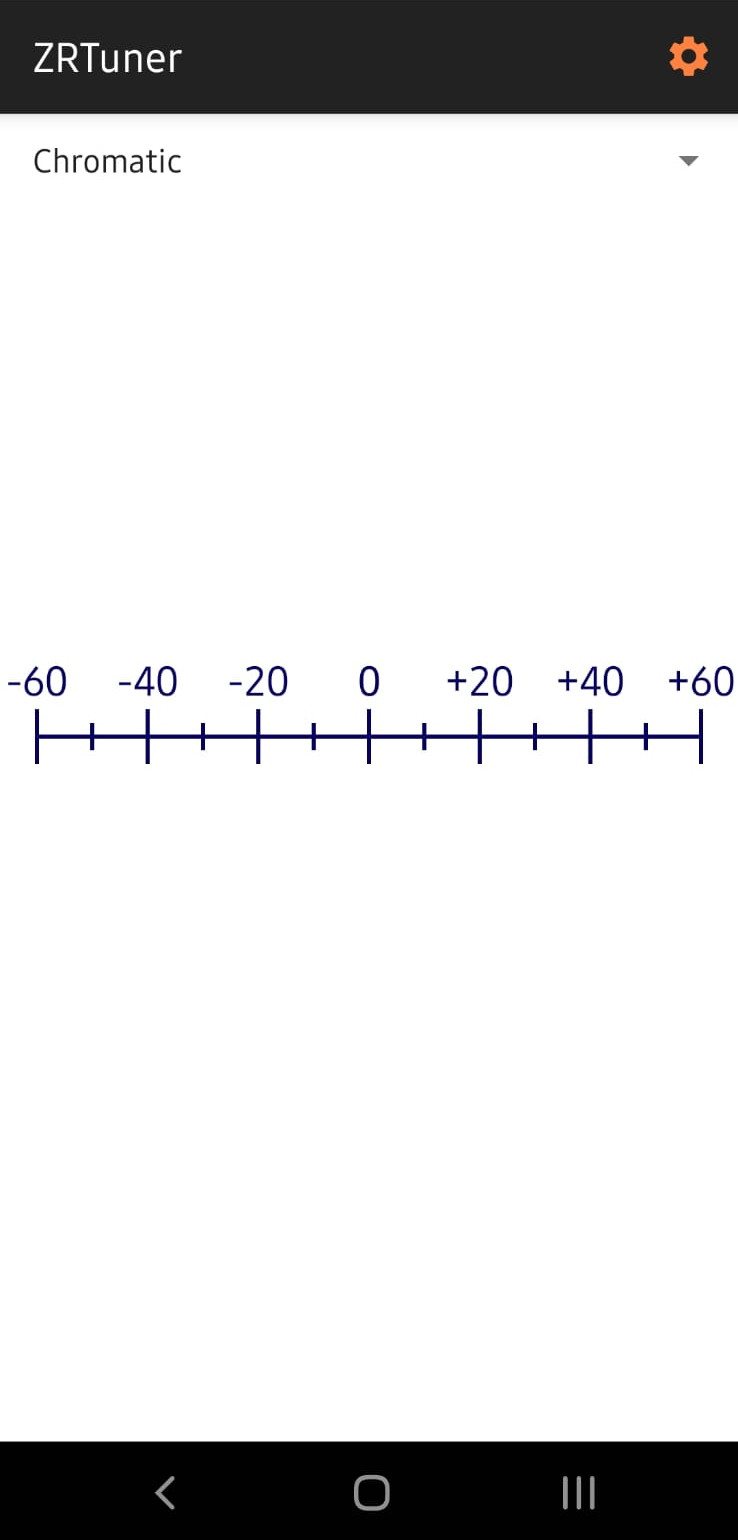
\includegraphics[height=0.9\textheight]{zrtuner_gauge.jpeg}}
	\caption{Početno sučelje aplikacije}
	\label{fig}
\end{figure}
\begin{figure}
	\centerline{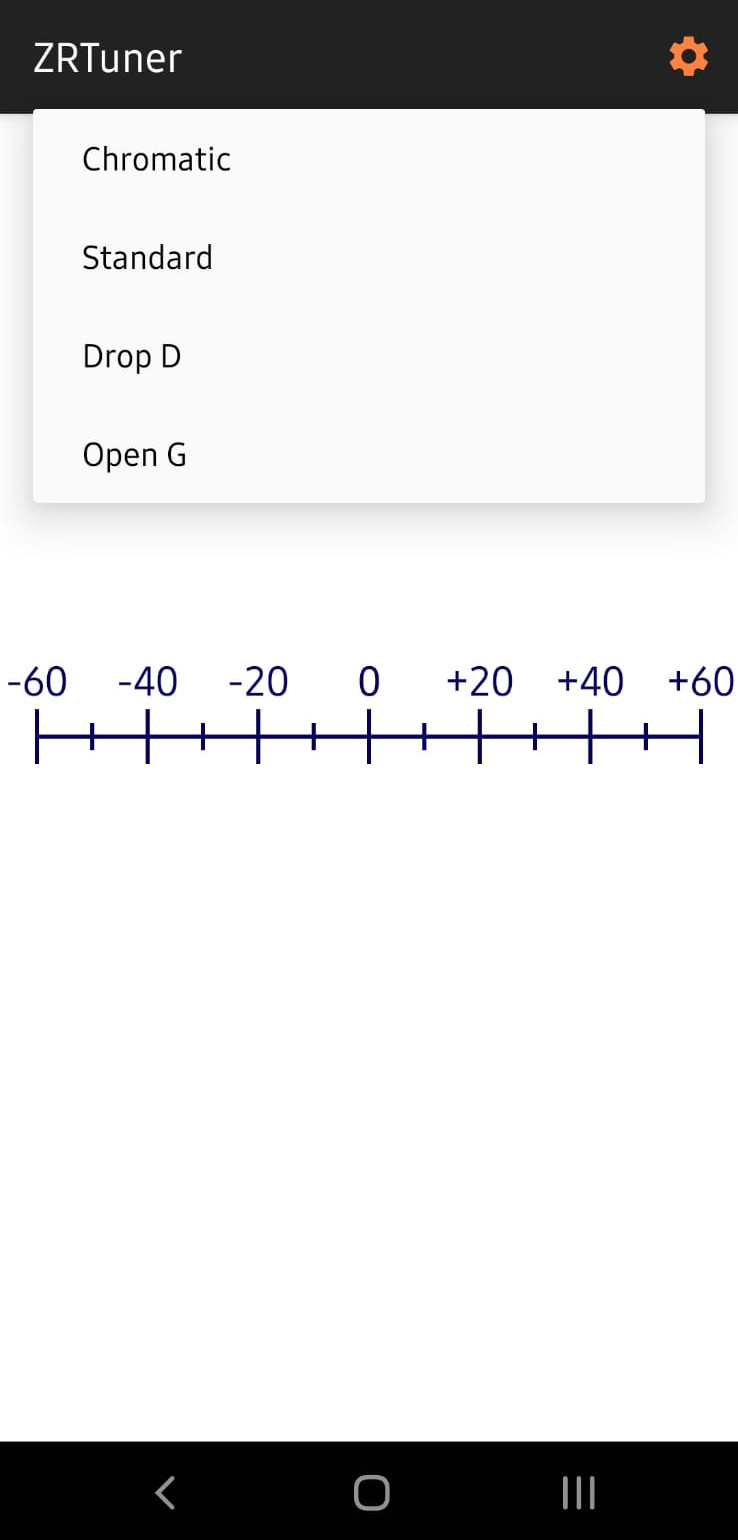
\includegraphics[height=0.9\textheight]{zrtuner_spinner.jpeg}}
	\caption{Sučelje padajućeg popisa načina štimanja}
	\label{fig}
\end{figure}
\begin{figure}
	\centerline{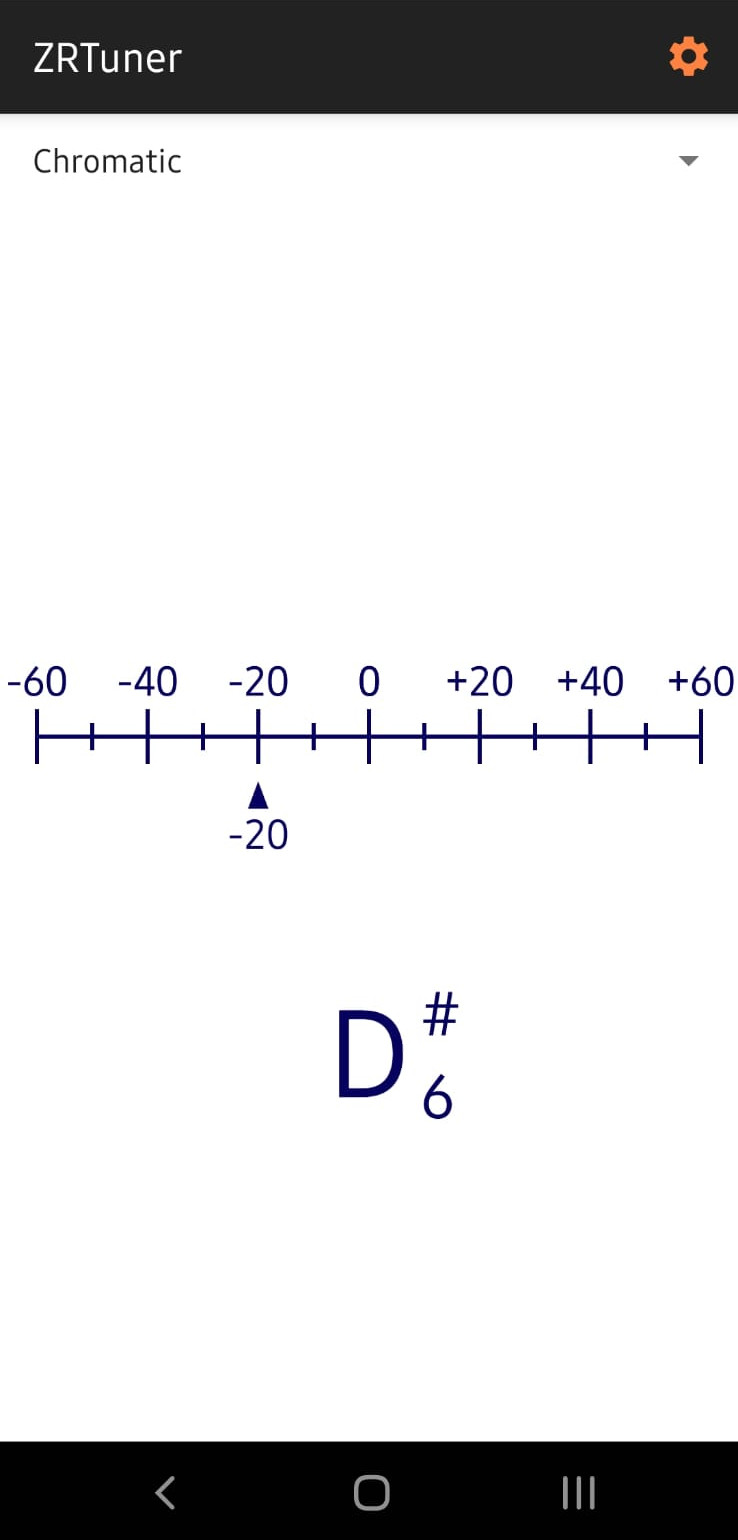
\includegraphics[height=0.9\textheight]{zrtuner_note.jpeg}}
	\caption{Sučelje mjerač pri prepoznatoj visini tona}
	\label{fig}
\end{figure}
\begin{figure}
	\centerline{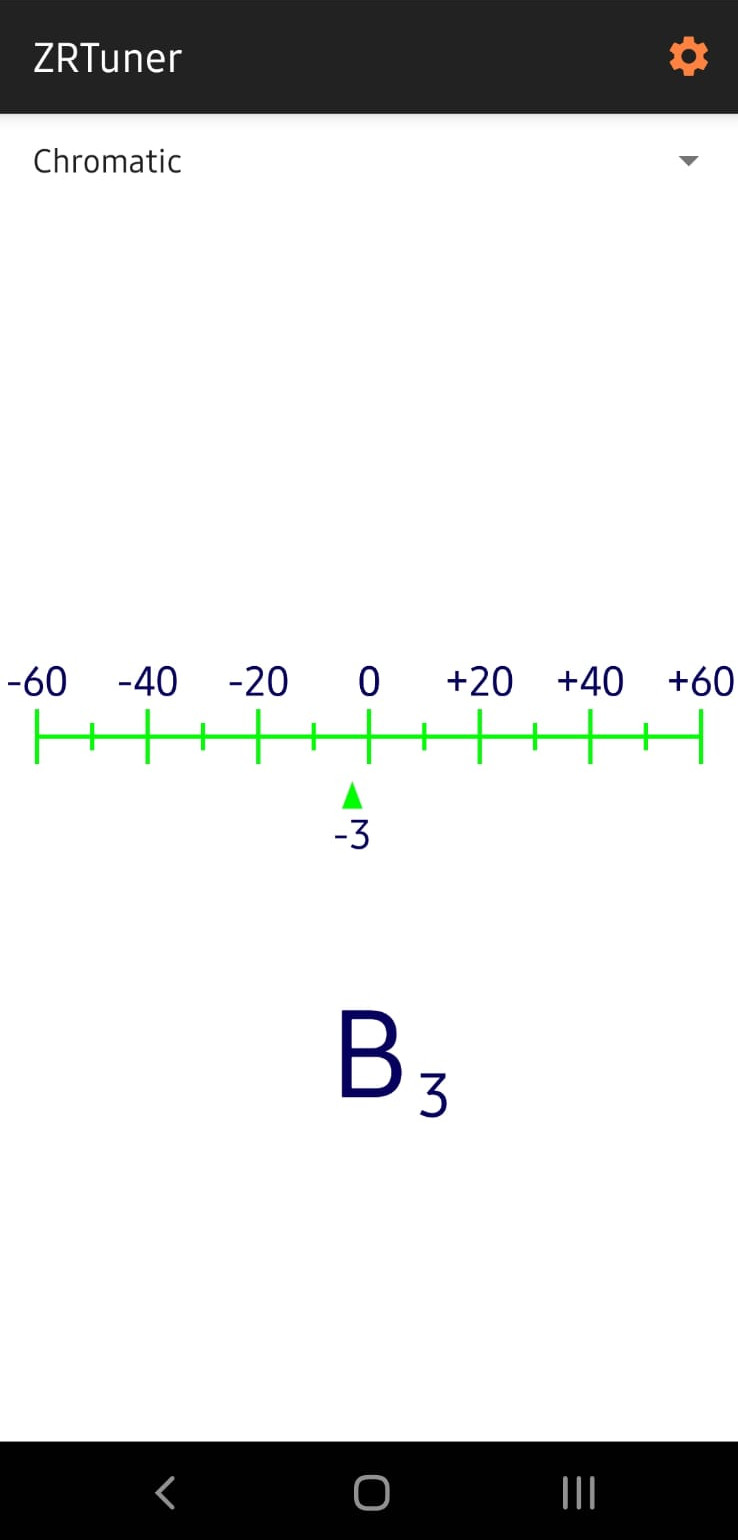
\includegraphics[height=0.9\textheight]{zrtuner_gauge_green.jpeg}}
	\caption{Sučelje mjerača pri maloj razlici u visinama tona}
	\label{fig}
\end{figure}
\begin{figure}
	\centerline{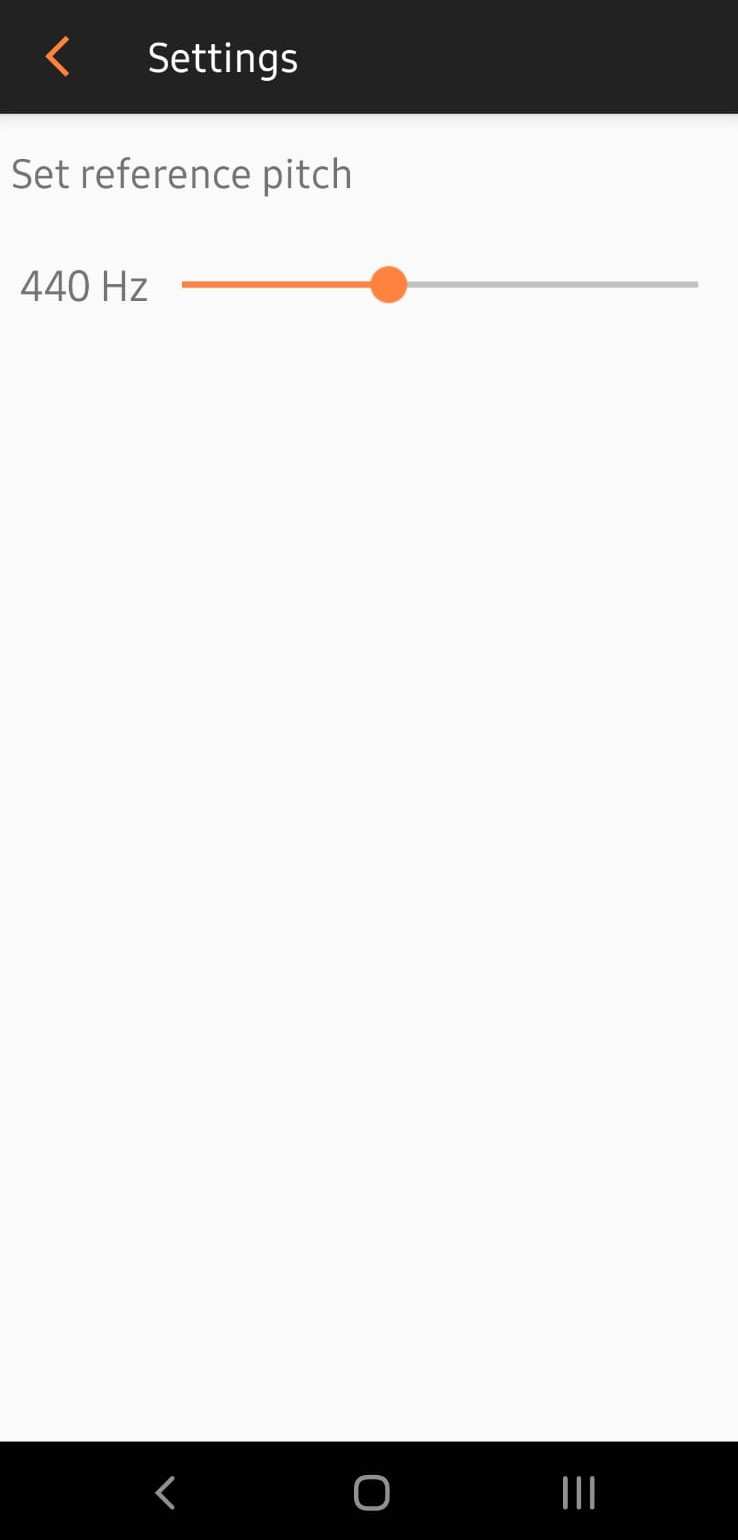
\includegraphics[height=0.9\textheight]{zrtuner_options_440.jpeg}}
	\caption{Sučelje postavki s klizačem za koncertnu visinu tona}
	\label{fig}
\end{figure}
\begin{figure}
	\centerline{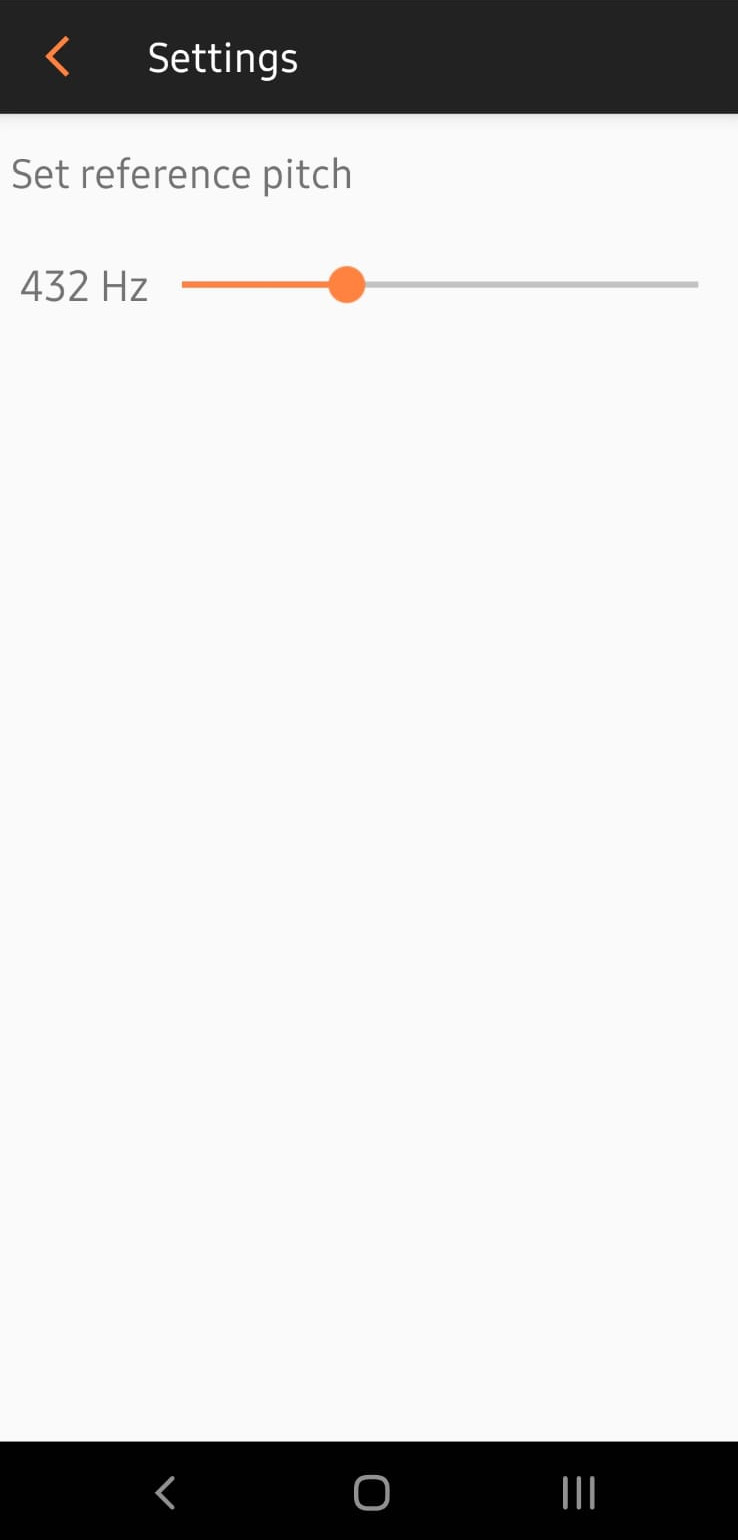
\includegraphics[height=0.9\textheight]{zrtuner_options_432.jpeg}}
	\caption{Sučelje postavki s promijenjenom koncertnom visionom tona}
	\label{fig}
\end{figure}

\clearpage

\section{Snimanje i obrada zvuka}
Aplikacija pri prvom dizanju šalje upit korisniku za dopuštenje snimanja zvuka. Dopuštenjem snimanja zvuka aplikacija kreće u rad, zove metodu \verb|startRecording()| u glavnoj klasi \verb|MainActivity| te pokreće snimanje i obradu zvuka.

\subsection{Stvaranje fragmenta}
Metoda \verb|startRecording()| instancira objekt klase \verb|FragmentManager| pomoću kojeg će moći instancirati i upravljati objektom klase \verb|ListenerFragment|\cite{gstraube}, koji će u sklopu klase \verb|MainActivity| služiti za pozivanje operacija potrebnih za detekciju visine tona. Aktivnosti (eng. \textit{Activity}) u Android aplikacijama najčešće su predstavljene kao prozori sa sučeljem koji su usredotočeni na obavljanje specifičnog zadatka.

Fragmenti u Android aplikacijama predstavljaju dio korisničkog sučelja s višekratnom uporabom koji služi za obavljanje specifičnih funkcija. Za dodavanje, brisanje i zamjenu fragmenata te upravljanje fragmentima koristi se klasa \verb|FragmentManager|. Klasa \verb|ListenerFragment| nasljeđuje klasu \verb|Fragment| te pomoću objekta klase \verb|FragmentManager| pri inicijalizaciji svog objekta dohvaća instancu svog fragmenta preko oznake "listener\_fragment".

Budući da pri prvome instanciranju fragment te oznake neće biti pronađen (jer još nije instanciran), uz pomoć metode \verb|beginTransaction()| započet će proces stvaranja novog fragmenta s oznakom "listener\_fragment". Metodom \verb|add()|, u glavnoj aktivnosti \verb|MainActivity| stvara se fragment \verb|ListenerFragment|, a metodom \verb|commit()| se taj proces izvršava i završava.

\clearpage
\renewcommand{\figurename}{Kod}
\begin{figure}
	\centerline{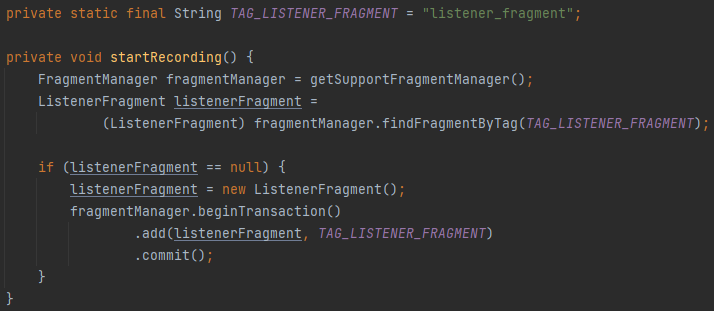
\includegraphics[width=\textwidth]{startRecording.png}}
	\caption{Stvaranje fragmenta za snimanje zvuka}
	\label{fig}
\end{figure}

\subsection{Pozadinski proces}
Stvaranjem fragmenta \verb|ListenerFragment| pokreće se instanca pozadinskog procesa privatne klase \verb|PitchListener|. \verb|PitchListener| nasljeđuje apstraktnu klasu \verb|AsyncTask| kako bi uz metodu \verb|doInBackground| aplikacija u pozadini mogla obrađivati snimljeni zvuk.

Metoda \verb|doInBackground| započinje instanciranjem objekta sučelja za rukovanje visinom tona \verb|PitchDetectionHandler| iz biblioteke TarsosDSP te lambda izrazom definira metodu \verb|handlePitch()|. 

!!!Boolean \verb|IS_RECORDING| u početnom je stanju \verb|false| te će se svaki put kada je u stanju \verb|false| izvršiti metoda \verb|publishProgress()|!!!

Klasom \verb|PitchDetectionResult| pomoću metode \verb|getPitch()| dohvaća se detektirana visina tona iz snimljenog bloka zvučnog signala. U slučaju detektirane visine tona instancira se objekt klase \verb|PitchDifference|, koji predstavlja devijaciju snimljene visine tona od njoj najbliže note. Objekt \verb|pitchDifference| preko klase \verb|PitchComparator| metodom \verb|retrieveNote()| dohvaća najbližu notu i devijaciju u visini tona izraženu u centima te ih kao objekt tipa \verb|PitchDifference| stavlja u niz \verb|pitchDifferences|. U trenutku kada se ovaj postupak ponovi barem \verb|MIN_PITCH_COUNT| puta (po potrebi izabrano 8 puta), izračunat će se prosječna visina tona niza \verb|pitchDifferences| te će metodom \verb|publishProgress()| ta vrijednost biti proslijeđena za prikaz korisniku.

Instanciranjem objekta \verb|pitchDetectionHandler|, njegova vrijednost prosljeđuje se kao argument za instanciranje objekta klase \verb|PitchProcessor| iz biblioteke TarsosDSP, zajedno s enumeracijom YIN algoritma \verb|FFT_YIN|, frekvencijom uzorkovanja \verb|SAMPLE_RATE| tipa \verb|int| i veličinom \textit{buffer}-a \verb|BUFFER_SIZE| tipa \verb|int|. 

Aplikacija koristi frekvenciju uzorkovanja od 44,1 kHz i veličinu \textit{buffer}-a od 4096 uzoraka. Time postiže rezoluciju od 10,77 Hz po uzorku, čime dobiva na brzini, ali gubi na preciznosti među najnižim frekvencijama u rasponu gitare. Ovaj kompromis je prihvatljiv budući da se mogućnost pojave grešaka pri nižim frekvencijama smanjuje na način da se uzastopno mjeri prosjek snimljenih blokova frekvencija. 

Klasa \verb|PitchProcessor| kao implementacija sučelja \verb|AudioProcessor| pruža funkcije namještanja izabranog algoritma za detekciju visine tona. U ovom slučaju se instancira objekt klase \verb|FastYin| koja u biblioteci TarsosDSP implementira YIN algoritam.

Iza instance \verb|pitchProcessor| instancira se objekt klase \verb|AudioDispatcher| koja služi za pretvorbu snimljenih zvučnih signala ili zapisa u obradive blokove. Za specifikaciju izvora zvuka koristi se metodama klase \verb|AudioDispatcherFactory|, u ovom slučaju metode \verb|fromDefaultMicrophone()|, budući da aplikacija obrađuje zvuk snimljen u stvarnom vremenu preko mikrofona na mobilnom uređaju. Kao argumenti joj se proslijeđuju \verb|SAMPLE_RATE|, \verb|BUFFER_SIZE| i veličina preklapanja \verb|OVERLAP| tipa \verb|int|. Veličina preklapanja u ovom slučaju je 3072 uzoraka, što je 75\% veličine \textit{buffer}-a (4096 uzoraka). Drugim riječima, svakih snimljenih 1024 uzoraka, započet će istovremeno snimanje novih 4096 uzoraka. Kao odabir procesora za obradu zvuka, \verb|audioDispatcher| postavlja \verb|pitchProcessor| metodom \verb|addAudioProcessor|. Konačno, snimanje i obrada signala započinje naredbom \verb|audioDispatcher.run()|.





\chapter{Zaključak}
%Zaključak.

\bibliography{literatura}
\bibliographystyle{fer}

\begin{sazetak}
%Sažetak na hrvatskom jeziku.

\kljucnerijeci{Ključne riječi, odvojene zarezima.}
\end{sazetak}

% TODO: Navedite naslov na engleskom jeziku.
\engtitle{Title}
\begin{abstract}
Abstract.

\keywords{Keywords.}
\end{abstract}

\end{document}
